\begin{savequote}[75mm]
The beginning is the most important part of the work.
\qauthor{Plato, The Republic}
\end{savequote}

% pending plagiarism check
\begin{flushleft}
\chapter{Image-based profiling of organoids}

\section{Disclosure}
Significant parts of this chapter have been adapted from own manuscripts, including \textit{The drug-induced phenotypic landscape of colorectal cancer organoids} \citep{Betge2022-kr}. The maximum contrast projection method, organoid segmentation method, feature extraction procedure and organoid viability classification (LDC) were previously developed by Jan Sauer as part of his dissertation \citep{noauthor_undated-ij}. Image-based profiling experiments were supported by Johannes Betge. 

\section{Establishing patient derived organoids for image-based profiling}

Patient derived organoids can be established from diverse set of healthy or malignant tissues and have been shown to represent their tissue of origin with respect to morphological and molecular features including gene expression and somatic mutations \citep{Fujii2016-ax, Weeber2015-sn, Van_De_Wetering2015-ko, Sato2011-lh,  Broutier2017-wg}. To generate personalized cancer models for image-based profiling, I designed and implemented a standardized laboratory workflow to generate patient derived organoids from colorectal cancer samples via endoscopic biopsy (Figure \ref{fig_110}a). Briefly, fresh patient samples were washed, digested and embedded in a basal membrane extract, a proprietary mixture of extracellular matrix proteins especially rich in Laminin and Collagen 4. The isolated tumor cells were then overlaid with a growth factor rich medium, containing Epidermal Growth Factor (EGF), the BMP-signaling antagonist Noggin and the small-molecule inhibitor A83-01, which inhibits TGF-beta-signaling by targeting the Activin receptor-like kinase family.

%\clearpage
\begin{figure}[h!]
\centering
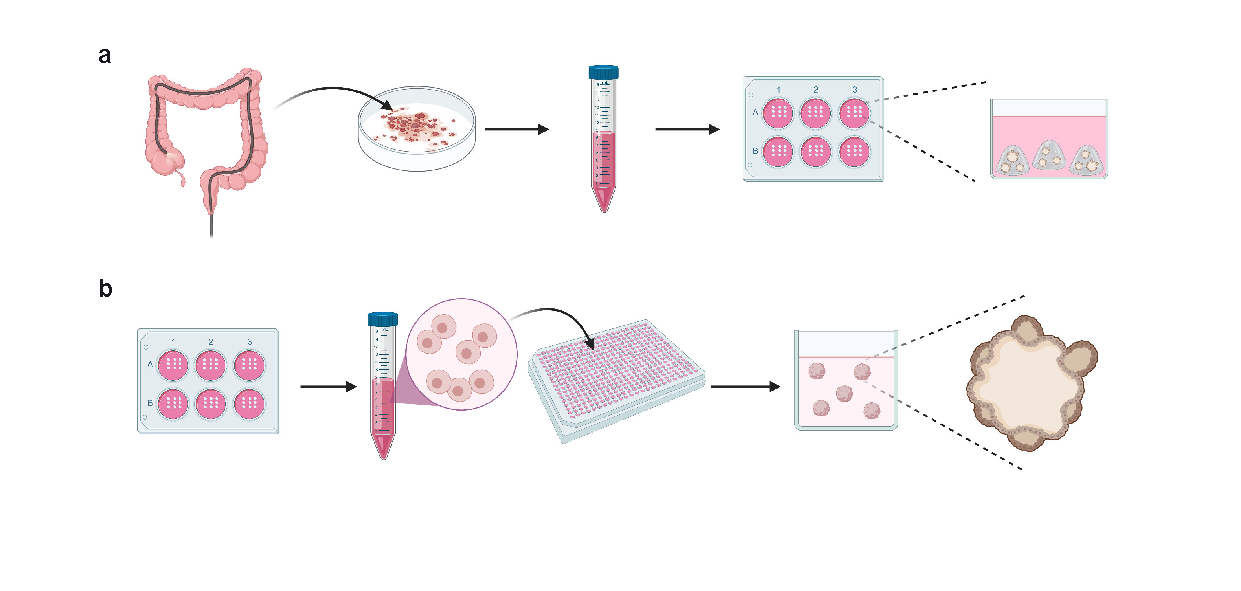
\includegraphics[width=\textwidth,
                height=\textheight,
                keepaspectratio]{figures/promise/pdf/fig_0_1.pdf}
\caption[Core organoid liquid handling methods]{\textbf{Core organoid liquid handling methods a} Organoid isolation procedure. Colorectal cancer tissue biopsies were collected via endoscopy, enzymatically removed from extracellular matrix proteins, washed and resuspended in basal membrane extract hydrogel. After solidification of hydrogel domes, organoids were overlayed with growth factor rich culture medium. \textbf{b} Organoid high-throughput experimentation. Colorectal cancer organoids were harvested, partially digested, seeded in hydrogel-coated 384-well plates}
\label{fig_110}
\end{figure}

\newpage
Following this protocol, patient derived organoids from 13 patients with colorectal cancer were prospectively developed. Donors to the biobank represented different UICC stages (Figure \ref{fig_120}a). 

\bigbreak
Amplicon sequencing of frequently altered genes in colorectal cancer showed molecular profiles characteristic for the disease (Figure \ref{fig_120}c). Similar to sequencing studies of primary tumors, patient derived organoids harbored a high frequency of APC (6/13), KRAS (8/13) and TP53 (5/13) mutations \citep{Muzny2012-hr}. 

\bigbreak
On a gene expression level, patient derived organoids mainly represented the canonical consensus molecular subtype CMS 2 of colorectal cancer \citep{Guinney2015-ex} (Figure \ref{fig_120}b). No patient derived organoid line with a MSI-high phenotype and the associated CMS 1 molecular subtype was established. Also, no organoid line matched the molecular subtype CMS 4, which is associated with stromal infiltration and TGF\(\beta\)-signaling. These results are in line with previous observations \citep{Van_De_Wetering2015-ko, Schutte2017-fl} and demonstrate limitations of the organoid culture system, which selects for growth of epithelial cells (favored by canonical Wnt signaling high, BMP4 signaling low) over mesenchymal cells (favored by canonical Wnt signaling low, BMP4 signaling high) \textit{ex vivo} \citep{Sato2011-lh}.

\clearpage
\begin{figure}[h]
\centering
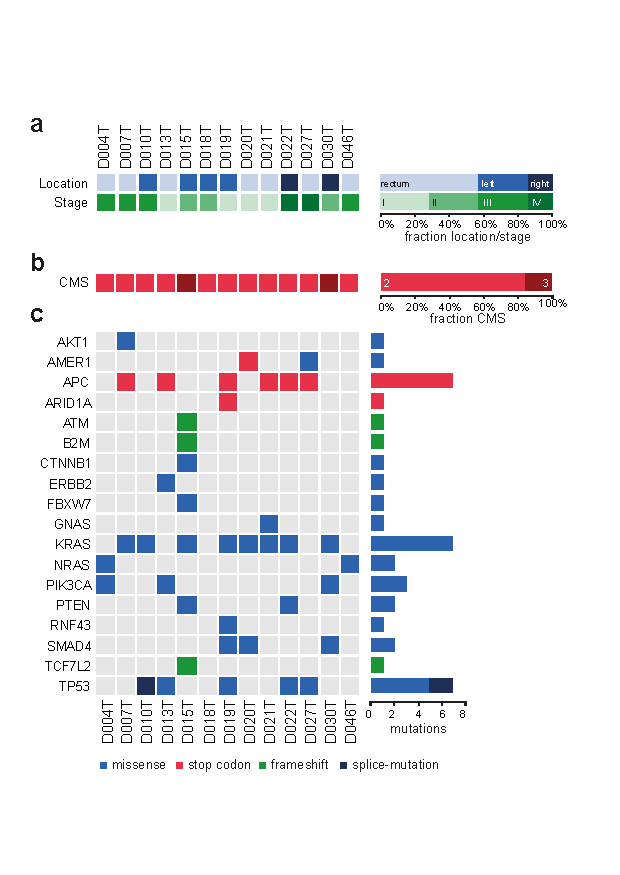
\includegraphics[width=\textwidth,
                height=\textheight,
                keepaspectratio]{figures/promise/pdf/fig_1_0.pdf}
\caption[Patient derived organoid cohort overview]{\textbf{Patient derived organoid cohort overview a} Tumor location (right/left/rectum) and AJCC/UICC stage of colorectal cancers that patient derived organoids were derived from. \textbf{b}  Consensus molecular subtypes of organoids determined by RNA expression analysis. \textbf{c} Mutation status in PDOs, as analyzed by amplicon sequencing. Figure created with support from Johannes Betge (graphical presentation),  Erica Valentini (sequencing data analysis) and Benedikt Rauscher (CMS type inference). Figure adapted from \textit{The drug-induced phenotypic landscape of colorectal cancer organoids} \citep{Betge2022-kr}}
\label{fig_120}
\end{figure}
\clearpage


\section{Enabling methods for high-throughput image-based profiling of organoids}
To systematically measure organoid morphology, I established a platform for high-throughput image-based profiling experiments (Figure \ref{fig_130}a). The three engineering problems that had to be solved were (1) control of organoid size and density in a 384-well plate format, (2) control of organoid location within the hydrogel for efficient microscopy and (3) maintenance of organoid integrity during automated fixation and permeabilization. 

\begin{figure}[h]
\centering
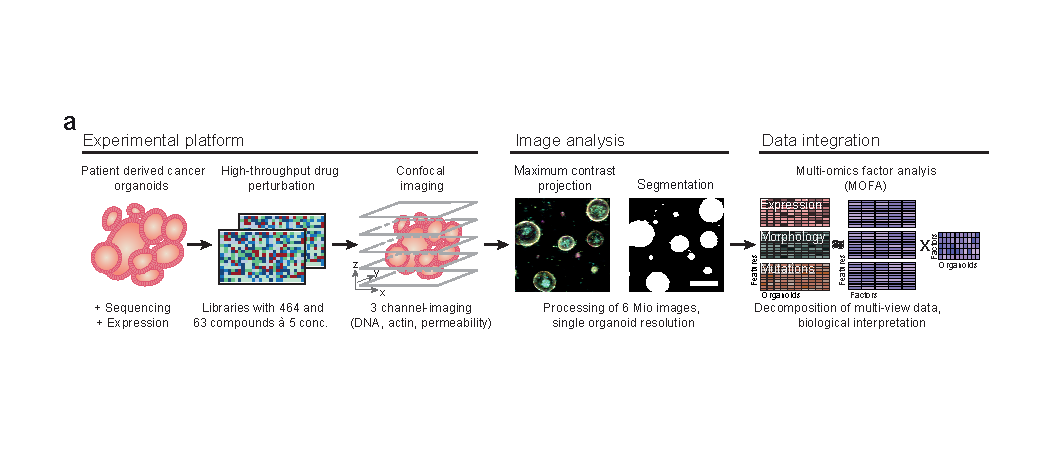
\includegraphics[width=\textwidth,
                height=\textheight,
                keepaspectratio]{figures/promise/pdf/fig_1_1.pdf}
\caption[Overview of multi-view profiling experiments]{\textbf{Overview of multi-view profiling experiments a} Organoids were isolated from endoscopic biopsies from patients with colorectal cancer. Organoids were dissociated and evenly seeded in 384-well plates before perturbation with an experimental (464 compounds) and a clinical compound library (63 compounds à 5 concentrations, 842 perturbations across both libraries). After treatment, high-throughput fluorescence microscopy was used to capture the morphology of organoids.  The multi-channel (DNA, beta-actin, cell permeability) 3D imaging data was projected, segmented, and descriptive features were extracted to quantify potential drug-induced phenotypes. Untreated organoid morphology, organoid size and drug activity scores were integrated with mRNA expression and mutation data in a Multi-Omics Factor Analysis (MOFA) to increase interpretability of organoid variation. Figure created with support from Johannes Betge (graphical presentation) and adapted from \textit{The drug-induced phenotypic landscape of colorectal cancer organoids} \citep{Betge2022-kr}}
\label{fig_130}
\end{figure}


A standard protocol for cell-based assays, including image-based profiling, is seeding cells into microwell plates at a fixed cell number. In order to determine cell number, adherent cells are dissociated and counted using optical methods. Patient derived organoids, however, demonstrated a low rate of organoid outgrowth when passaged by complete organoid dissociation down to the single cell level. To improve organoid outgrowth, the dissociation protocol was stopped early, yielding cell clusters of ca. 1-10 cells. These organoid fragments showed an increased outgrowth rate, which could be further improved by treating cells with 10 μM of Rho-Kinase inhibitor Y-27632 (data not shown). To control organoid size and density, organoids were digested with a modified trypsin derivative, and filtered through a 40 um cell strainer to ensure an upper limit of organoid fragment size. To effectively estimate the cell number while maintaining organoid fragments, organoid fragments were titrated based on their ATP concentration, instead of cell count. The ATP concentration of the organoid fragment suspension was determined using an ATP-dependent luminescence readout. After controlling for ATP concentration, the organoid fragment suspension was seeded onto basal membrane extract covered 384 well plates.

\begin{figure}[h]
\centering
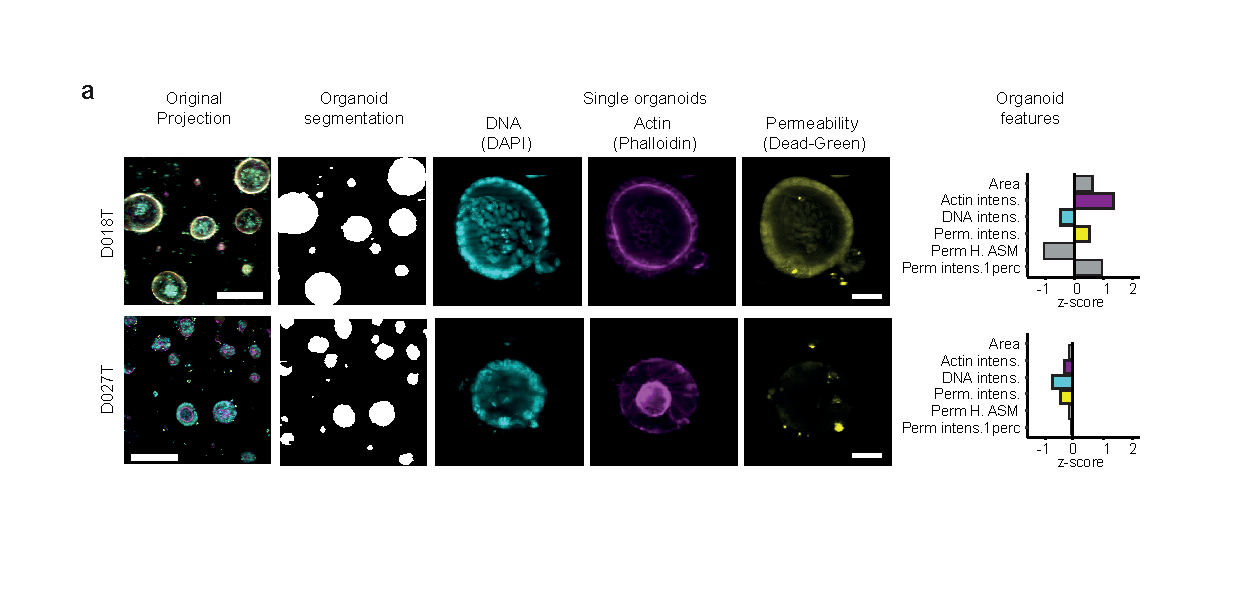
\includegraphics[width=\textwidth,
                height=\textheight,
                keepaspectratio]{figures/promise/pdf/fig_1_2.pdf}
\caption[Image-based profiling method overview]{\textbf{Image-based profiling method overview a} The image-processing pipeline illustrated with representative example images from two organoid lines: Organoids were imaged at multiple layers along the z-axis. Images were projected using a maximum contrast projection and segmented using a convolutional neural network, both designed and implemented by Jan Sauer. Descriptive features were extracted from all three channels to quantify phenotypes. Feature plots show the median phenotype of unperturbed organoids, six example features (Area, Phalloidin intensity, DAPI intensity, FITC intensity, FITC Haralic angular second moment (ASM) and FITC intensity 1-percentile) and their z-scores relative to all profiled organoid lines are shown. Figure created with support from Jan Sauer (data processing) and Johannes Betge (graphical presentation). Figure adapted from \textit{The drug-induced phenotypic landscape of colorectal cancer organoids} \citep{Betge2022-kr}}
\label{fig_135}
\end{figure}

\bigbreak

Conventional image-based profiling of adherent cells is based on automatic microscopy of one 2D plane per field of view. Given the 3D growth patterns of organoids, more data has to be acquired to fully capture organoid phenotype. Acquiring multiple planes of imaging data per field of view, however, creates a technical data storage and processing burden. For a fixed 3D volume, the dimensions of the collected data increase linearly with the number of acquired planes and quadratically with the target z-axis resolution. To reduce the observed 3D volume and thus the number of required imaging planes, the vertical distribution of organoid fragments within the basal membrane extract layer was controlled by centrifuging organoid fragments post-seeding at 500G for 20 minutes at 37 degrees Celsius. The centrifugal force led to an accelerated sedimentation of organoid fragments onto the same optical plane before the polymerization of the hydrogel was complete.

\bigbreak

After three days of culture and four days of compound treatment, organoids were fixed and stained for actin (Phalloidin/TRITC), DNA (DAPI), and cell permeability (DeadGreen/FITC) (Figure \ref{fig_135}a). Subsequently, plates were imaged at multiple z-positions by automated confocal microscopy. During treatment with the hyperosmolar fixative (3\% para-formaldehyde in phosphate buffered saline) the protein rich hydrogel underwent an irreversible volume contraction (data not shown). To reduce this artefact, the fixative was supplemented with bovine serum albumin to a final concentration of 1\% weight/volume. After image acquisition, 3D data was projected into a 2D plane by applying a maximum contrast projection followed by segmentation with a weakly-supervised convolutional neural network and single-organoid-level feature extraction (Figure \ref{fig_135}a). In summary, seeding well-quantifiable organoid fragments instead of single cells, centrifuging organoid fragments to reduce the imaged 3D volume, and modifying liquid handling buffers to avoid hydrogel-driven artefacts technically enabled high-throughput image-based profiling of organoid models. 

\end{flushleft}
